%!TEX root = cscw2019-comic.tex
\section{Method}
\label{sec:Method}
In this study, we examined if the abstract comic can impact a decision with monetary consequence on Amazon Mechanical Turk. The persuasion task is to ask participants to make a charitable donation decision to the Organization for Autism Research with the real money. 

\textcolor{red}{In this section, we will first discuss the choice of task, then show how we construct persuasive messages (\Cref{sub:Constructing Persuasive Messages}). Then, we introduce our experimental design (\Cref{sub:Experiment Design}), discuss study procedure (\Cref{sub:Study Procedure}) and participant recruitment (\Cref{sub:Participant Recruitment}).}

%How should we decide on the experimental context in which we could examine the effects of the abstract comic form in stimulating behavior? There are many different compelling behavioral contexts: personal wellness goals (e.g., diet, exercise), mundane tasks (e.g. ``pick up dry cleaning''), as well as broader public-goods issues (e.g. ``take the flu shot;'' ``donate to cure cancer'')

\subsection{Choice of Task: Charitable Donation}
\label{sub:Choice of Task: Charitable Donation}


There are many different compelling behavioral contexts on which to test the role of the comic form: personal wellness goals (e.g., diet, exercise), mundane tasks (e.g. ``pick up dry cleaning''), as well as broader public-goods issues (e.g. ``take the flu shot;'' ``donate to cure cancer'').

\textcolor{red}{We identify four criteria consistent with prior literature \cite{lee2013does, sussman2015framing,saunders2016no,rumsey2003influence} to guide us, in our choice of the experimental behavioral context: nature of the reward; single shot tasks; an ecologically valid task; absence of specialized knowledge to perform the task. First, we would like the rewards to be distant, and non-exclusive, rather than proximal and exclusive so that individuals don't perform the task in anticipation of the immediate reward. Thus public goods dilemmas (e.g. ``reducing carbon footprint;'' ``taking the flu shot''; ``contributing to public knowledge'') are all candidates. Second, while some longitudinal tasks (e.g., losing weight; eating healthy) have distant rewards (losing weight, or maintaining a diet takes time), and can positively affect the public good (with more healthy people, in the long-run, insurance rates will fall), these tasks are prone to habit formation, a potential confound. Furthermore, single-shot tasks such as ``pick up yogurt at the grocery store today'', often prompted by text reminders from our calendars or task-tracking apps, have an immediate, exclusive reward. Third, we would like to ensure that the experimental task is ecologically valid---a task that these individuals would be actually asked to perform in the wild, outside of the experimental context. Fourth, we would like the task not to require specialized knowledge (e.g. ``asking doctors to make a decision''), so that other researchers could easily replicate and scale our experiment. }


Online charitable donation tasks satisfy these criteria as they are single-shot tasks, contribute to the public good with distant, non-exclusive rewards, requests for charitable donations frequently occur online, and the task allows for experimental replication. 

\textcolor{red}{We also considered two other in-the-wild experimental scenarios. First, we considered the task of persuading individuals to buy healthy food by sending them push notifications on the smartphone, when they were shopping for groceries. We encountered three challenges. First, we could not control for confounds in the decision making (discounts on salad / healthy items; if the shopper was in a rush; they were shopping with friends who were pursuing a healthy lifestyle). Second, what would be the size of the social network (to help determine the social norm) of friends of each experimental subject would we include? The size of social circles on platforms like Facebook is typically large. Third, the reward had a possible confound?for some participants, healthier food may make them feel better, and thus they may make the choice to buy the healthier food not because of the message, but because of the anticipated reward. Second, instead of purchase donation decisions, we considered persuading individuals to adopt healthy behaviors, such as talking a walk, or going to the gym. Then, we would count the number of times a subject conducted a behavior rather than quality (that is, count the number of gym visits instead of measuring the effectiveness of the activity in the gym). The central challenge here is that these activities are prone to habit formation, a confound. If habit forms, it may be more important in causing repeated behavior than the message received. With all considerations, we chose online charitable donations tasks in our study} 

In our study, we choose the Organization for Autism Research (OAR) for three reasons. First, Autism Spectrum Disorder (ASD), is a well-known developmental disorder that impairs communication and behavior \cite{american2013diagnostic}; ASD provides basic interest for the participants to support the related charitable organization. Second, the Organization for Autism Research is one of the most visible ASD related organizations that helps individuals with autism and provides assistance to their parents, families, teachers, and caregivers. The goal of OAR is clear and reputable so participants won't question the authenticity of our message's motive. Finally, we wished to avoid a charity associated with a life-threatening condition such as cancer as it may create an experimental confound: we don't know if someone donates because their intrinsic desire to help with a life-threatening situation. While ASD can have serious consequences on the well being of those who have it, the public perception is that ASD is not-life threatening. 

% In other words, ASD provides basic interest for the participants to support the related charitable organization. 


% \subsection{Choice of Charity: Organization for Autism Research (OAR)}



% We chose OAR as the charity in our study for three reasons. First, Autism Spectrum Disorder (ASD), is a well-known, developmental disorder which provides basic interest for the participants to support the related charitable organization. Second, the Organization for Autism Research is one of the most visible ASD related organizations that helps individuals with autism and provides assistance to their parents, families, teachers, and caregivers. The goal of OAR is clear and reputable so participants won't question the authenticity of our message's motive. Finally, we wished to avoid a charity associated with a life-threatening condition such as cancer as it may create an experimental confound: we don't know if someone donates because their intrinsic desire to help with a life-threatening situation. While ASD can have serious consequences on the well being of those who have it, the public perception is that ASD is not-life threatening. 



%We chose a charity associated with Autism (Organization for Autism Research) for our experiment.



%As we mentioned in earlier sections, four design principles guided us to choose the online charitable donation task. First, the online charitable donation is a kind of collective dilemma where study participants will receive distant rewards based on their decision, which signifies the impact from the persuasive message. Second, encouraging people to donate is a single shot task that requires no habit formation, which protects us from several confounding factors such as life events and resource constraints (e.g., time). Third, with the advance in social network and internet, although the task is still challenging, charities or organizations nowadays solicit donations online textual messages (e.g., Wikipedia's fundraising banner), which makes our task ecologically valid. Fourth, online charitable donation requires no specialized knowledge. In our study, we choose the Organization for Autism Research since Autism Spectrum Disorder (ASD), is a well-known developmental disorder that impairs communication and behavior \cite{american2013diagnostic}. In other words, ASD provides basic interest for the participants to support the related charitable organization. In this section, we will introduce the experiment design and describe our participants recruiting process.

%In this study, we examine if the abstract comic can impact a decision with monetary consequence. The aim of this study is to show the persuasiveness of the abstract comic in the real-life setting.  
%In contrast, the first study demonstrated that participants prefer messages in abstract comic form over text, but did not demonstrate persuasiveness.
% as more persuasive, it is unknown if the perceived persuasiveness can impact people's real-life decision making. So, we further studied the ability of abstract comics in persuading people to make decisions in real life. 
% In the second study, we conduct a field study on Amazon Mechanical Turk and compared the power between pure text messages and abstract comic messages in persuading people to donate with their real money. 
%In this section, we will introduce the experiment design and describe our study participants recruiting process.


\subsection{Experiment Design}
\label{sub:Experiment Design}
Since the main goal for this study is to compare the power of a persuasive message in two forms, the abstract comic and the text, we first constructed two experimental conditions, the comic condition (see~\Cref{fig:basic three comic panel}) and the text condition. In the comic condition, participants will read a message asking if they are willing to support a charity in a three-panel abstract comic strip, whereas in the text condition, participants will receive the same message in plain text form. 

To test the idea of social proof, we then added a third condition, the comic with the social proof condition. Participants will read a three-panel comic strip that has the same content as the comic condition but added one line text indicating the normative behavior (see~\Cref{fig:basic three comic social proof}). To gather the basic statistics to create social proof, we first ran a pilot study with the first two conditions ($n=60$) and used the donation statistics as part of the social proof message. In the pilot study, 87\% of the participants donated a non-zero amount. 
% Additionally, we are also interested in if the abstract comic can leverage persuasive techniques to increase its persuasiveness. Hence, we incorporated the idea of social proof and created the third condition, social-proof-comic.

\begin{figure}[bt]
    \centering
    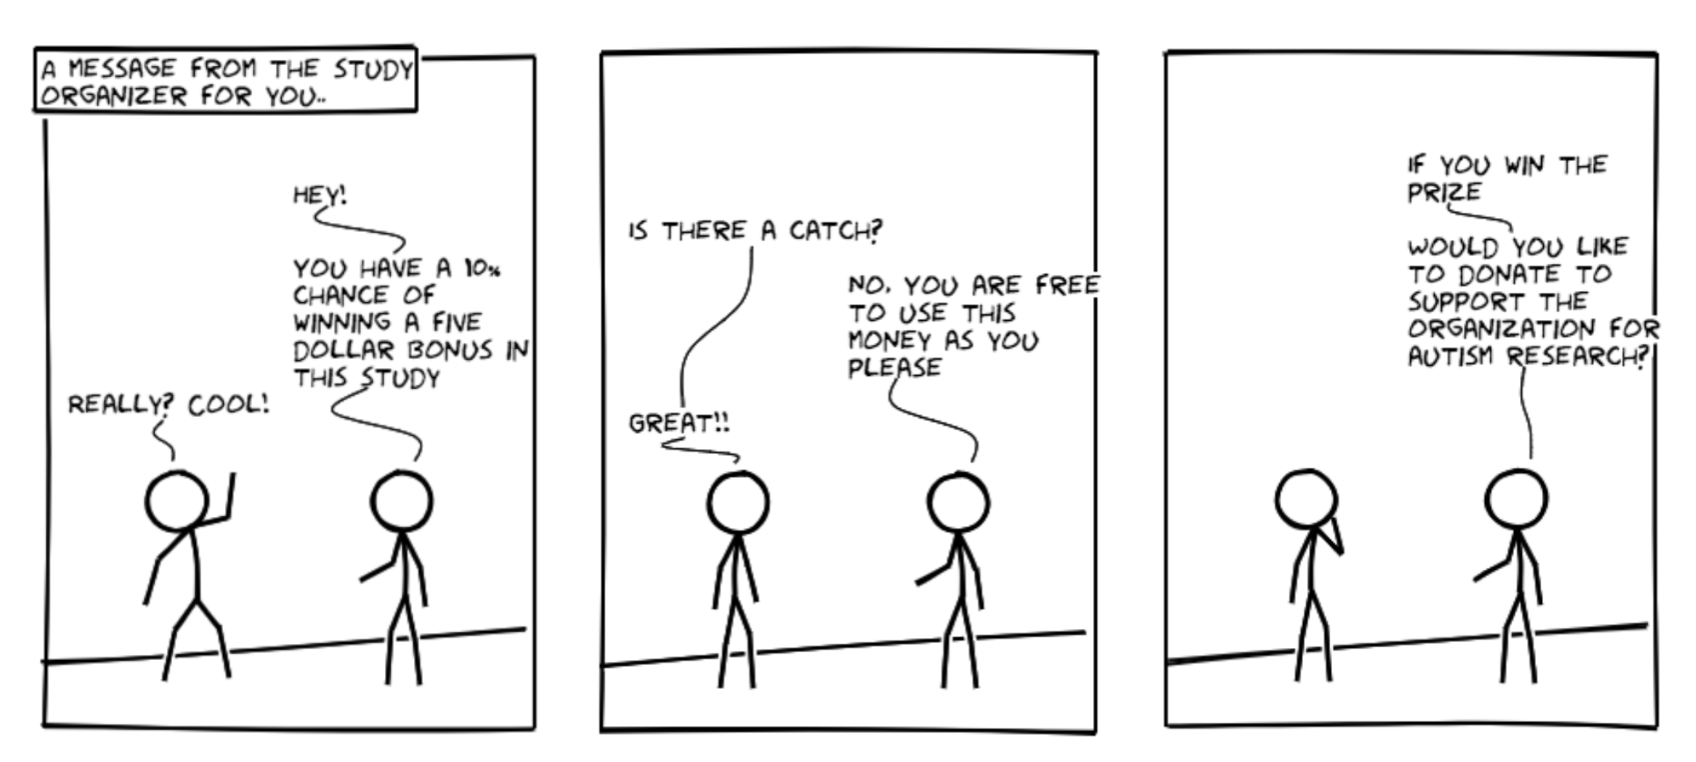
\includegraphics[width=\columnwidth]{./figures/abstract_comic.png}
    \caption{Messages in the abstract comic form. Same as the text messages, the three-panel comic strip communicates three points: 1) Participants will have 10\% of a chance winning \$5 bonus upon the completion of the study (see the first panel); 2) Participants are free to use the money as they please (see the second panel); 3) Participants can donate this bonus to the Organization for Autism Research (OAR) (see the third panel).}
    \label{fig:basic three comic panel}
\end{figure}

The objectives of the persuasive message in all three conditions are the same: persuading participants to donate to a charity from his/her own pocket. \textcolor{red}{Similar to \textcite{lee2013does,saunders2016no}, the money participants will use is part of their study reward, a prospective bonus reward (10\% chance of winning \$5 bonus).} We randomly assigned study participants to one of the three conditions; the participants are free to make a decision on the amount of donation, including not donating at all.




\subsection{Constructing Persuasive Messages}
\label{sub:Constructing Persuasive Messages}

% \subsubsection{Generating Comics}
% \label{sub:Generating Comics}



% \subsubsection{Message Content}
% \label{sub:Message Content}

Now we discuss construction of the three different messages: a plain text message, a comic, and a comic with social proof. Each message communicates three points: 1) Participants will have 10 \% of a chance winning \$ 5 bonus upon the completion of the study. 2) Participants are free to use the money as they please. and 3) Participants can donate this bonus to the Organization for Autism Research (OAR). Therefore, in the text condition, study participants will read the following message,
\begin{quote}
  \textit{You have a 10\% chance of winning a five dollar bonus in this study. You are free to use this money as you please. If you win the prize, would you like to donate to support the Organization for Autism Research?}
\end{quote}

In the two comic conditions, we created three-panel comic strips to communicate the \textit{same} text message. We used three panels to communicate each of the three points in the message. 

\textcolor{red}{While aesthetic considerations govern the choice of the number of panels in the comic form, two factors influenced choice of the number of panels: the number of points in the message, and communicating the idea of a conversation, over time, between two individuals. We wish to communicate three points (chance of winning bonus; free to use the money as they please; voluntary donation) in the short comic, and to ensure that each point was salient, we chose to communicate each point in a different panel. Comic panels along with the text bubbles within a panel fragment time and space. Time flows in two ways: vertically in each panel through the dialogue between the characters and across panels. Since this is a short conversation, three panels seemed appropriate. While adding more panels would elongate the perceived sense of time, we wished to be economical in our communication of the interaction between two characters. We can control of the number of panels in our software (see~\Cref{sec:Discussion}), and we leave the question of how the number of panels (and thus the perceived sense of time) affects message comprehension for future work.}

\textcolor{red}{To help the reader connect across panels to achieve closure~\textcite[][Chapter 3]{scott1993understanding} suggests that it is essential to match the panels. Different techniques to match exist, including ``moment-to-moment'', ``action-to-action'', ``scene-to-scene'' etc. helping the reader bridge different time scales (see~\parencite[][p. 71]{scott1993understanding} for a summary). We used the ``action-to-action'' matching technique~\cite{scott1993understanding} since all the activity occurs in one scene, and where the activity depicts a brief dialogue between two characters. In particular, we matched the panels on the gesture of the first character (the message recipient), while retaining a neutral gesture for the second character (who delivers the message). }



% The three-panel comic strip allows us to leverage one of the most fascinating aspects of comics---storytelling~\cite{scott1993understanding}. 
%Since the first study did not show a convincing effect for framing, participant gesture, character distance and shading, we did not vary those conditions in this experiment. We set the inter-character distance to be medium, light background. 
Consistent with ``match on action'' technique~\cite{scott1993understanding}, we matched the panels on the gesture of the first character (the message recipient), while retaining a neutral gesture for the second character (who delivers the message). 

%We create the comic strip in a manner similar to the first study on preference.

% Each of the three panel communicates one major objective in the message. The comic strip is created in the similar fashion as in the first study on preference. As we learned from the first study that appropriate gestures will maximize the persuasiveness of the comics, we then chose the gesture that we believe best suit for the scenario see~\Cref{fig:basic three comic panel}.

In the comic with social proof condition, we created social-proof by adding one sentence on the last comic panel indicates the percentage of people in our study donated(\Cref{fig:basic three comic social proof}). The percentage (87\%) corresponds to the number of people who donated a non-zero amount in the pilot study.


For the purposes of this study, we created a comic generator to generate comic strips used in the study. The generator leveraged an open source comic library, ``cmx.io'' ~\cite{cmx.io}, to generate comic figures and used ``rough.js'' \cite{rough.js} to generate other elements such as text bubbles and outline frames. The generator impersonates the style found on ``XKCD''~\cite{munroe2009xkcd} comic. Our focus is not the XKCD style, but the fact that the generated comic is abstract. We believe the generator has the potential to be further developed as a general framework to automatically synthesize pure-textual persuasive messages into abstract comic forms (we discuss this aspect further in section ~\Cref{sec:Discussion}).


% \begin{figure*}
%  \subfloat[Messages in the abstract comic form]{%
%   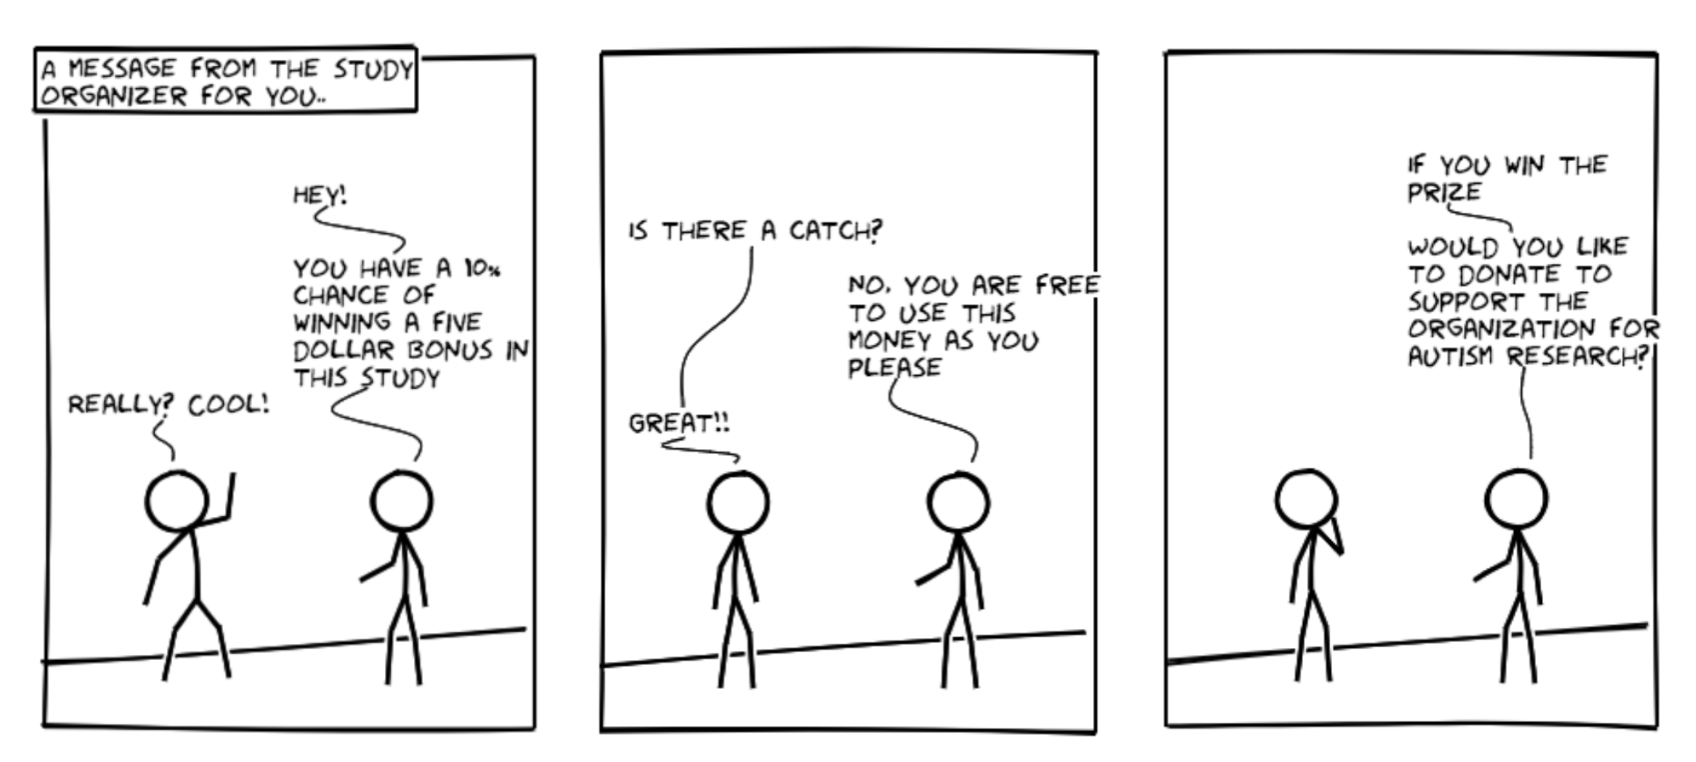
\includegraphics[width=0.5\textwidth]{./figures/abstract_comic.png}
%   } \hfill
%  \subfloat[Messages in the abstract comic form with social proof]{%
%   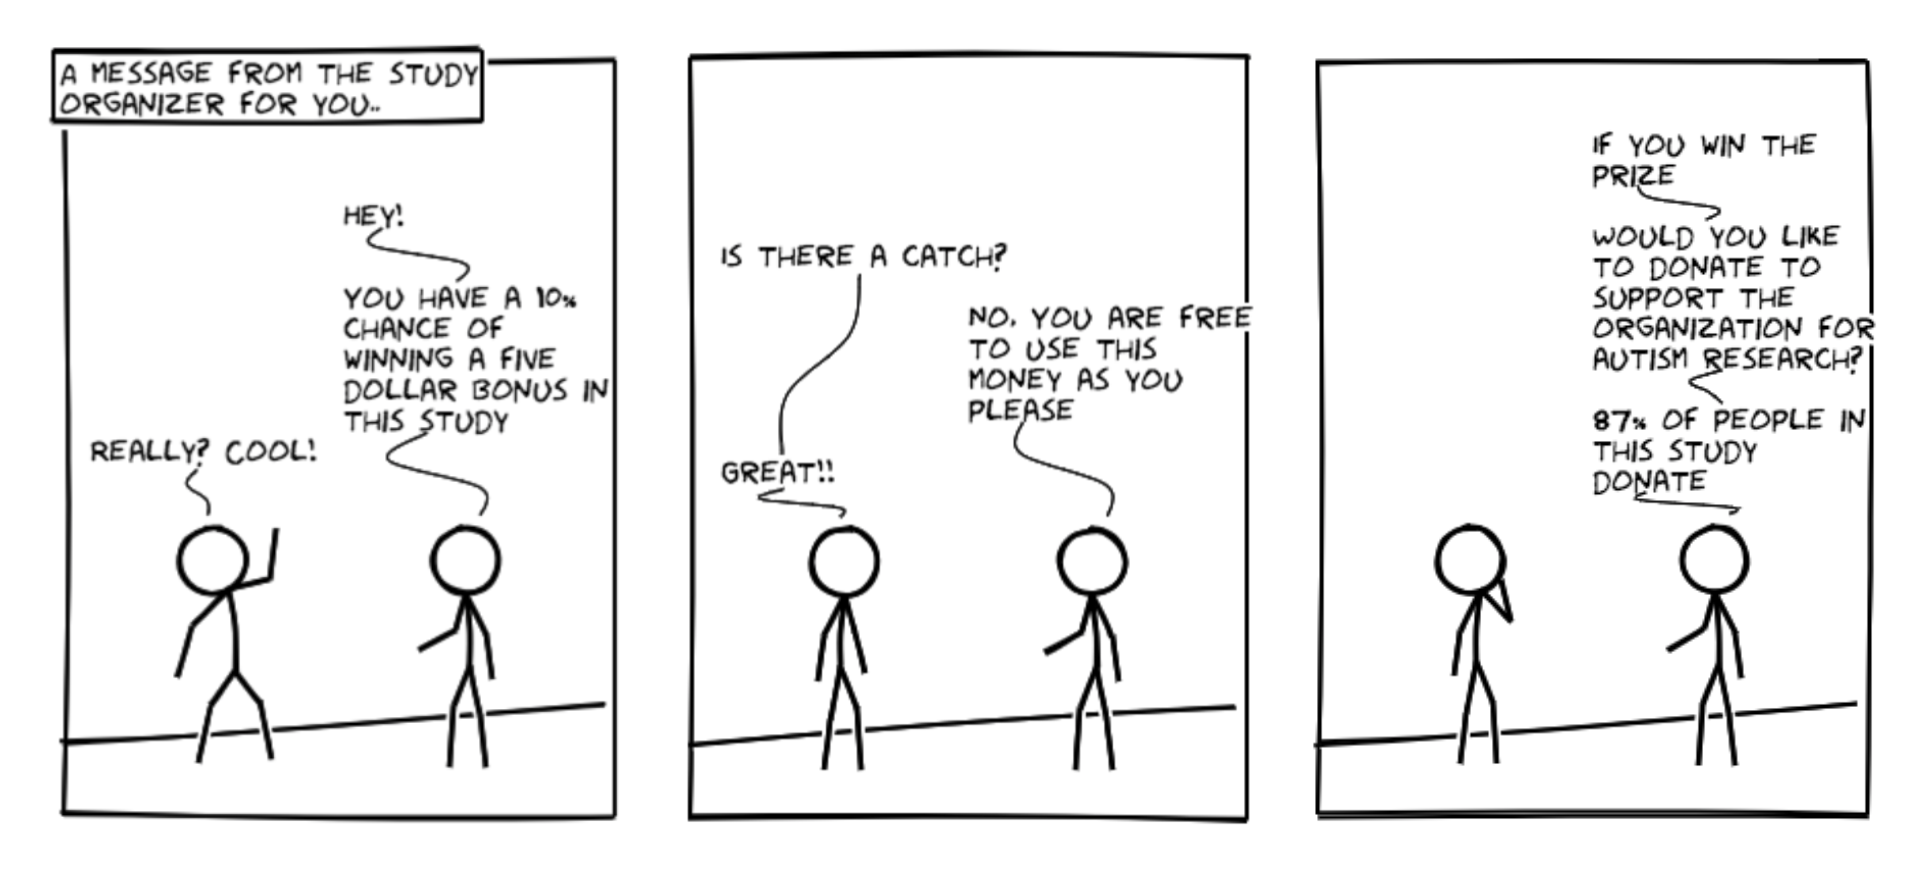
\includegraphics[width=0.5\textwidth]{./figures/social_proof.png}
%  }
%  \caption{The messages participants received in two abstract-comic conditions}
%  \label{fig:comic_messages_in_two_conditions}
% \end{figure*}


\subsection{Study Procedure} 
\label{sub:Study Procedure}
Once participants consented to join the study, we ask them if they are familiar with the Autism Spectrum Disorder (ASD). Then, each participant watched a short video produced by the Organization for Autism Research that promotes its fundraising activity "RUN FOR AUTISM" ~\cite{youtube_research}. After watching the video, we asked participants to summarize the video using free text and ask them to provide their opinion about the effectiveness of the video. The recruiting message specifically mentioned this task of soliciting their opinion on video message's effectiveness. \textcolor{red}{There are two main goals for this part of the study: first, similar to the informational materials (e.g. text) used in other donation studies \cite{lee2013does,10362981,FEILER20121322}, the video provides context. we want to make sure prior familiarity with autism do not confound our study; second, we want our main task less intrusive as soliciting charitable donation is not a common task on Amazon Mechanical Turk. We did consider establishing context by other means, such as an informative page with text and images on the organization of autism research. We decided against such an approach, because we could not guarantee that all subjects would have read the page. Furthermore, making subjects answer questions about the web-page to check if they had read the page carefully, seemed artificial, impinging on ecological validity. Finally, the linearity of the video is an advantage: subjects could advance to the next page only after watching the video, ensuring consistent knowledge to the best of our ability, on part of all participants.}

We then randomly assigned participants to one of the three conditions and then asked them to read the corresponding persuasive message (text, three-panel comic, three-panel comic with social proof). In the message, we provided the participant with a 10\% chance of winning \$5 additional bonus reward. We also provided them with the opportunity to donate to the Organization for Autism Research (OAR) which is the charity mentioned in the video they previously watched. 

\textcolor{red}{To best demonstrate the persuasiveness of the message itself, in our messages, we made it clear to participants that they can use the bonus freely as they please. The donation is completely voluntary and irrelevant to the compensation. The default donation amount for everyone is set to \$0 to control for the default effect.} Similar to ~\textcite{lee2013does}, we also diffused the responsibility of donation amount among all participants. Before the participants make their decision, they read ``The total amount of money allocated to [the charity] by all the winning participants will be aggregated and donated at the end of the study.'' Then, we asked the participants to decide the amount of money they are willing to donate on a slider bar with \$0 and \$5 as two extreme ends. The default position of the slider bar is at the \$0 end. To increase the realism of our study, the donation decision is not hypothetical: the winning participants receive the amounts that they choose keep; as study organizers we donate to the Organization for Autism Research (OAR) the cumulative sum of the participant donations. 

Before leaving the study, Participants to filled a demographic questionnaire about their gender, income and education; the participants had the option of declining to state an answer for each question.

At the end of the study, we randomly chose 10\% of the participants, donated to OAR based on their decision, and rewarded them with part of the bonus that they wished to keep.




\begin{figure}[bt]
    \centering
    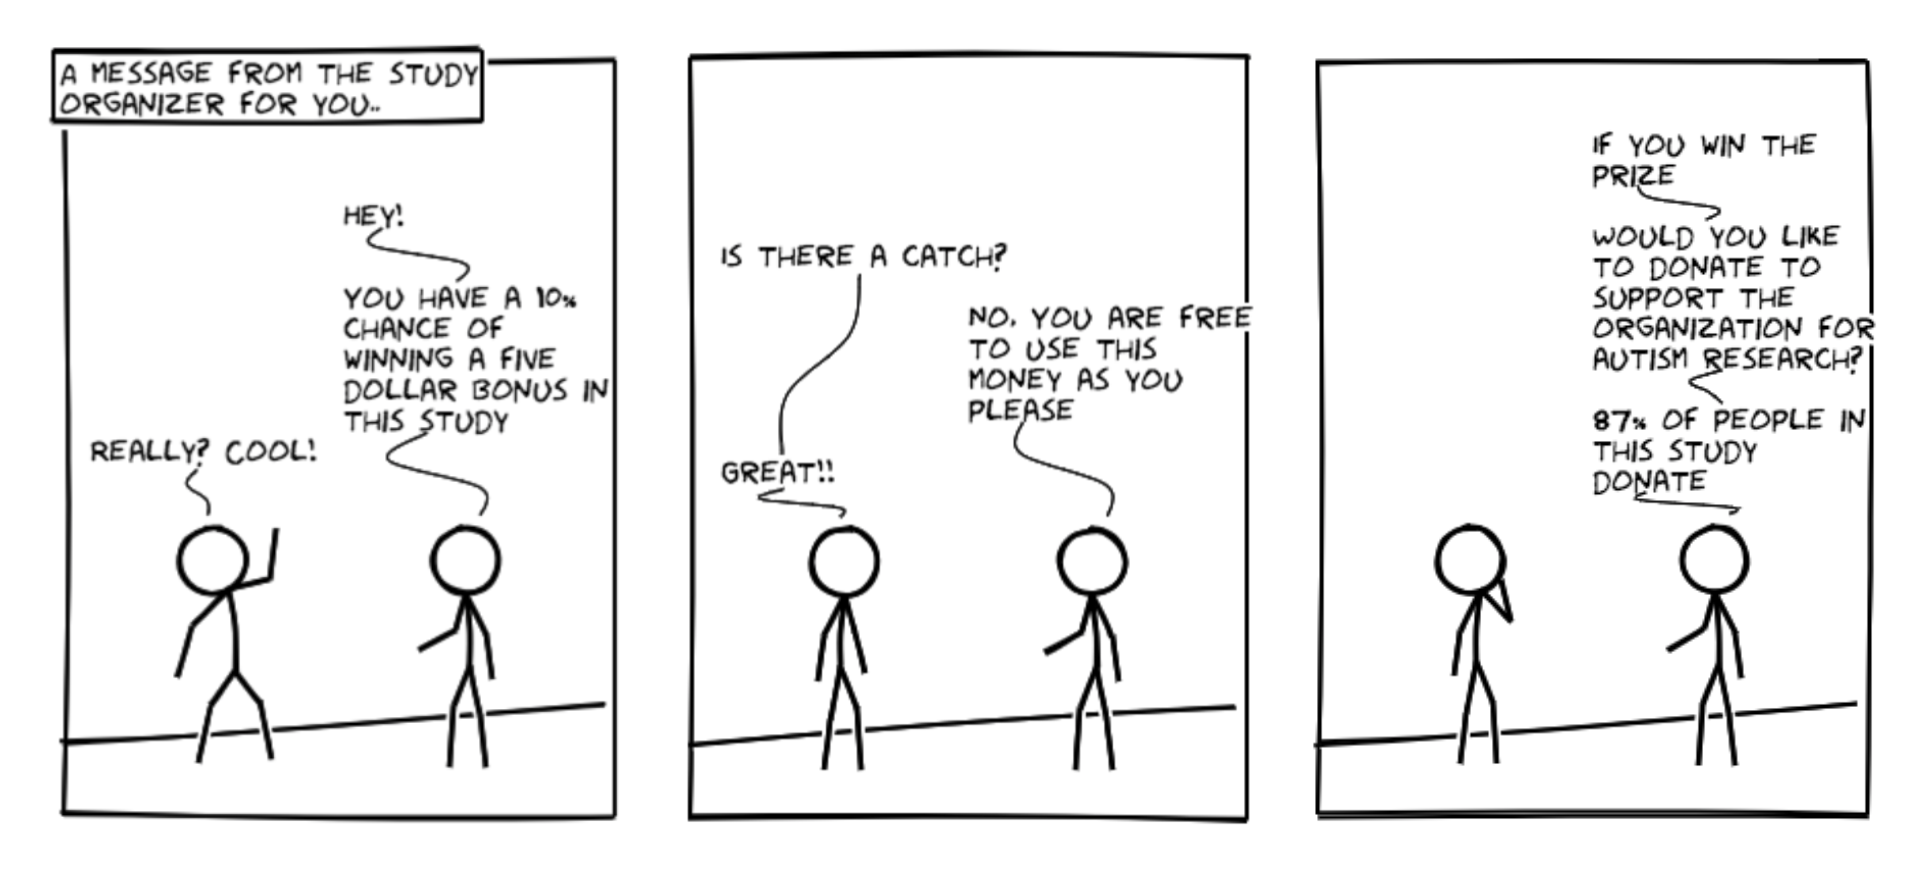
\includegraphics[width=\columnwidth]{./figures/social_proof.png}
    \caption{Messages with social proof. In addition to the three points that we wish to communicate (chance of winning bonus; free to use the money as they please; voluntary donation), the comic with social proof communicates the idea of the social proof at the third comic panel. The figure ``87\%'' comes from our pilot study}
    \label{fig:basic three comic social proof}
\end{figure}



\subsection{Participant Recruitment}
\label{sub:Participant Recruitment}
In this study, we recruit our study participants from Amazon Mechanical Turk. Although Amazon Mechanical Turk is a crowdsourcing platform that has been widely used to gather human intelligence in AI research and social science experiments \cite{ paolacci2014inside,berinsky2012evaluating,buhrmester2011amazon,branas2018gender,lee2013does,saunders2016no,arechar2017turking,sussman2015framing}, we should be cautious when using such platform as the participant selection criteria is not transparent \cite{landers2015inconvenient,paolacci2010running}. In our study, we chose the Amazon Mechanical Turk for the following reasons. First, our persuasion task is about online charitable donation which targets internet users. Second, crowdsourcing platforms will help us reach a more diverse sample than using the researchers' own social network to attract participants \cite{buhrmester2011amazon}. Third, the main motive for Amazon Mechanical Turk workers is monetary rewards \cite{berinsky2012evaluating}. In our study design, people will more sensitive to the monetary reward they may get and carefully make the donation decision, which makes our persuasive message more crucial. \textcolor{red}{Forth, multiple studies on charitable donation decisions have solicited donations from Amazon Mechanical Turk users\cite{branas2018gender,lee2013does,saunders2016no,arechar2017turking,sussman2015framing}. Fifth, Amazon Mechanical Turk is public accessible. Although working with a non-profit organization may strengthen results, working with a non-profit is that the experiment is harder to replicate by other researchers, who may lack access to the same non-profit.} Thus, we believe it is valid for our experiment to use Amazon Mechanical Turk as our sample pool. 

Motivated by studies that show that populations on Amazon Mechanical Turk are diverse and mirror the US population \cite{buhrmester2011amazon,behrend2011viability,berinsky2012evaluating}, we recruited our participants from Amazon Mechanical Turk. However, we are aware of research that raises concerns in Amazon Mechanical Turk's sample representativeness \cite{landers2015inconvenient,paolacci2010running}. One potential solution is to use a panel company's population (e.g., Qualtrics). However, this method also has concerns in that the researcher can not directly cross-validate the sample's representativeness we have to trust the company's assertion.

We published our HITs on Amazon Mechanical Turk titled ``A short survey about communicating autism campaign ads``. The compensation was \$10/hr, and the workers would get these rewards regardless of their performance. To ensure quality, the HIT is limited to English Speakers and people who have a 95\% Approval Rate. On the HIT page, we instructed that repeated responses would be rejected. We told the participants that they would see a link to our experiment site. 
